\chapter{Cristalografía y difracción de rayos X}\label{ch:b3:x-ray-diffraction}

En 1912, un haz de rayos X enviado a través de un cristal de sulfato de cobre dejó en una
placa fotográfica un patrón de manchas nítidas: los cristales difractan los rayos X como una
red difracta la luz, porque las distancias entre sus átomos son
comparables a la longitud de onda de los rayos X. Un año después, William Lawrence Bragg, entonces
estudiante, leyó en esos patrones la estructura de la sal gema ---y mostró que
el sólido no contiene en absoluto moléculas de \ce{NaCl}, sino solo una red en la que cada ion
tiene seis vecinos del otro tipo. Todas las estructuras cristalinas citadas en el
volumen del primer año y en este libro se determinaron así. Este capítulo da la
geometría de las redes y de su simetría, la condición de difracción, las
intensidades que revelan el contenido de la celda, y los métodos de polvo y de
monocristal que se usan en todos los laboratorios.

\begin{recall}
El volumen del primer año describió los cristales mediante una red de nodos, un motivo y una
celda unidad con sus parámetros de red; contó la multiplicidad de una celda; construyó
las estructuras cúbica centrada en las caras, cúbica centrada en el cuerpo y hexagonal compacta,
y los tipos sal gema, cloruro de cesio, blenda y fluorita; y calculó una densidad a partir de una celda.
El \cref{ch:b3:point-groups} definió las
\omterm{def:b3:point-groups:operation}{operaciones de simetría} y los \omterm{def:b3:point-groups:point-group}{grupos puntuales}.
\end{recall}

\begin{omfigure}
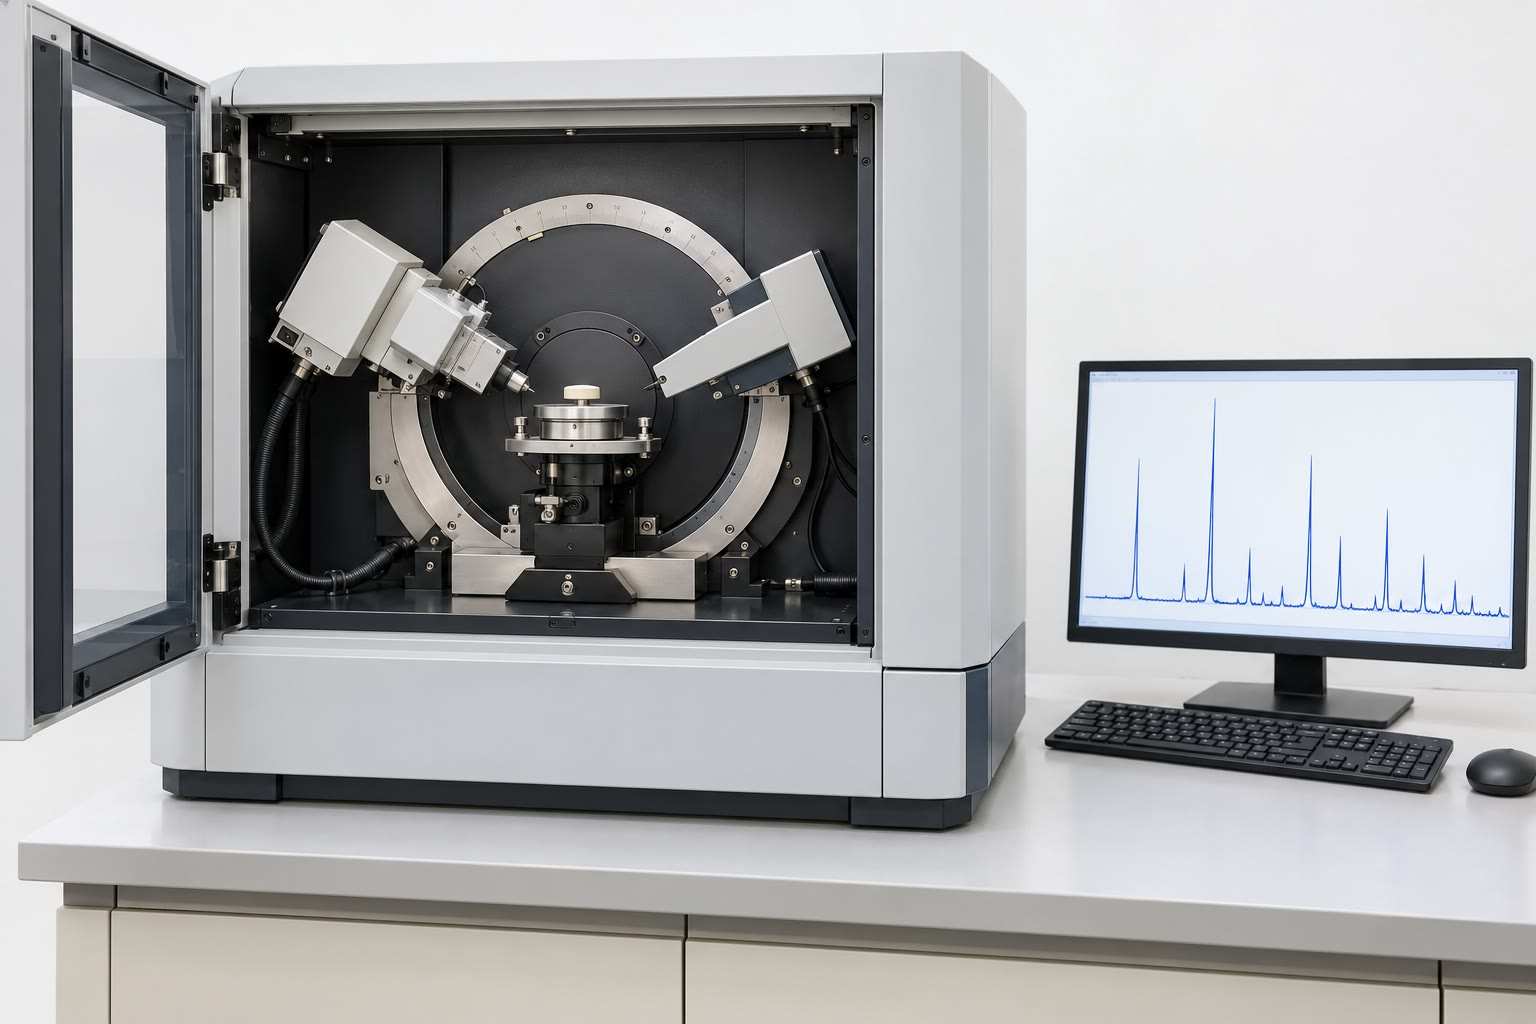
\includegraphics[width=0.6\linewidth]{images/book4/ai/b3-09-diffractometer.jpg}

{\small Un difractómetro de polvo de sobremesa: el tubo de rayos X y el detector
giran sobre un círculo en torno a la muestra plana.}
\end{omfigure}

\section{Sistemas cristalinos y redes de Bravais}

Una red solo puede tener \omterm{def:b3:point-groups:operation}{operaciones de simetría} que transformen la red en sí misma.
Eso las restringe mucho.

\begin{theorem}[La restricción cristalográfica]\label{thm:b3:x-ray-diffraction:restriction}
Los únicos ejes de rotación compatibles con una red son de orden 1, 2, 3, 4 y 6.
\end{theorem}

\begin{proof}
En una base de vectores de la red, una rotación de simetría transforma vectores de la red en
vectores de la red, de modo que su matriz tiene coeficientes enteros y traza entera. La
traza no depende de la base; en una base ortonormal con $z$ según el
eje vale $1 + 2\cos\theta$. Por tanto, $2\cos\theta$ es un entero entre $-2$ y 2:
$\cos\theta \in \{-1, -\frac12, 0, \frac12, 1\}$, $\theta = 180^\circ, 120^\circ, 90^\circ,
60^\circ, 0^\circ$: órdenes 2, 3, 4, 6, 1. Un eje de orden cinco es imposible.
\end{proof}

\begin{definition}[Sistema cristalino, red de Bravais, centrado de la red]\label{def:b3:x-ray-diffraction:crystal-system}
Las redes se agrupan según su simetría en siete \emph{sistemas
cristalinos}\index{sistema cristalino} (triclínico, monoclínico, ortorrómbico, tetragonal,
trigonal, hexagonal, cúbico). Una celda puede tener nodos de la red solo en sus vértices
(primitiva, P) o también en su centro (centrada en el cuerpo, I), en los centros de todas las
caras (centrada en las caras, F) o de un par de caras (centrada en las bases, C), o a lo largo de una
diagonal del cuerpo (romboédrica, R): es su \emph{centrado de la
red}\index{centrado de la red}. Las 14 combinaciones distintas de un sistema y
un centrado son las \emph{redes de Bravais}\index{red de Bravais}.
\end{definition}

\begin{center}\small
\begin{tabular}{lll}
\hline
sistema & restricciones de la celda & centrados \\ \hline
triclínico & ninguna & P \\
monoclínico & $\alpha = \gamma = 90^\circ$ & P, C \\
ortorrómbico & $\alpha = \beta = \gamma = 90^\circ$ & P, C, I, F \\
tetragonal & $a = b$, todos los ángulos de $90^\circ$ & P, I \\
trigonal & $a = b = c$, $\alpha = \beta = \gamma \ne 90^\circ$ (ejes romboédricos) & R \\
hexagonal & $a = b$, $\alpha = \beta = 90^\circ$, $\gamma = 120^\circ$ & P \\
cúbico & $a = b = c$, todos los ángulos de $90^\circ$ & P, I, F \\ \hline
\end{tabular}
\end{center}

\begin{omfigure}
\tdplotsetmaincoords{60}{100}
\begin{tikzpicture}[tdplot_main_coords, scale=1.25, font=\small]
  \foreach \s/\lab in {0/{cúbica P}, 3.0/{cúbica I}, 6.0/{cúbica F}}{
    \begin{scope}[xshift=\s cm]
      \pic[transform shape] {omcubeo={1.6}};
      \foreach \x in {0,1.6}{\foreach \y in {0,1.6}{\foreach \z in {0,1.6}{\node[cellA=2.6mm] at (\x,\y,\z) {};}}}
      \node[anchor=north] at (0.8,0.8,-0.62) {\lab};
    \end{scope}}
  \begin{scope}[xshift=3.0cm]
    \node[cellB=2.6mm] at (0.8,0.8,0.8) {};
  \end{scope}
  \begin{scope}[xshift=6.0cm]
    \foreach \p in {(0.8,0.8,0),(0.8,0.8,1.6),(0.8,0,0.8),(0.8,1.6,0.8),(0,0.8,0.8),(1.6,0.8,0.8)}{\node[cellB=2.6mm] at \p {};}
  \end{scope}
\end{tikzpicture}

{\small Las tres \omterm{def:b3:x-ray-diffraction:crystal-system}{redes de Bravais} cúbicas: primitiva (nodos en los vértices),
centrada en el cuerpo (más el centro, en rojo) y centrada en las caras (más los seis centros
de las caras, en rojo). Sus celdas contienen 1, 2 y 4 nodos.}
\end{omfigure}

\section{Planos reticulares y red recíproca}

\begin{definition}[Plano reticular, índices de Miller, distancia interplanar]\label{def:b3:x-ray-diffraction:miller}
Un \emph{plano reticular}\index{plano reticular} es un plano que pasa por al menos tres
nodos no alineados; pertenece a una familia de planos paralelos y equidistantes
que contienen todos los nodos. Si el plano de la familia más próximo al origen corta
los ejes en $a/h$, $b/k$, $c/l$, los enteros $(hkl)$, sin factor común,
son sus \emph{índices de Miller}\index{indices de Miller@índices de Miller} (un índice 0 para un plano
paralelo a un eje). La distancia entre planos adyacentes es la
\emph{distancia interplanar}\index{distancia interplanar} $d_{hkl}$.
\end{definition}

\begin{proposition}[Distancias en celdas ortogonales]\label{prop:b3:x-ray-diffraction:spacing}
Para una celda ortorrómbica, $\dfrac{1}{d_{hkl}^2} = \dfrac{h^2}{a^2} + \dfrac{k^2}{b^2} +
\dfrac{l^2}{c^2}$; para una celda cúbica, $d_{hkl} = a/\sqrt{h^2 + k^2 + l^2}$.
\end{proposition}

\begin{proof}
El plano $hx/a + ky/b + lz/c = 1$ tiene vector normal $\mathbf n = (h/a, k/b, l/c)$
y está a la distancia $1/|\mathbf n|$ del origen; el plano paralelo que pasa por
el origen pertenece a la familia, luego $d = 1/|\mathbf n|$.
\end{proof}

\begin{definition}[Red recíproca]\label{def:b3:x-ray-diffraction:reciprocal}
Para una red de vectores de base $\mathbf a$, $\mathbf b$, $\mathbf c$ y volumen de celda $V$,
la \emph{red recíproca}\index{red reciproca@red recíproca} tiene los vectores de base
$\mathbf a^* = (\mathbf b\times\mathbf c)/V$, $\mathbf b^* = (\mathbf c\times\mathbf a)/V$,
$\mathbf c^* = (\mathbf a\times\mathbf b)/V$, de modo que $\mathbf a\cdot\mathbf a^* = 1$ y
$\mathbf a\cdot\mathbf b^* = 0$. Su nodo $\mathbf G_{hkl} = h\mathbf a^* + k\mathbf b^* + l\mathbf c^*$ es
perpendicular a los planos $(hkl)$, y $|\mathbf G_{hkl}| = 1/d_{hkl}$.
\end{definition}

\section{Difracción}

\begin{theorem}[Ley de Bragg]\label{thm:b3:x-ray-diffraction:bragg}
Los rayos X de longitud de onda $\lambda$ se reflejan en una familia de planos de distancia $d$
solo a los ángulos rasantes $\theta$ que cumplen
\[
2d\sin\theta = n\lambda, \qquad n = 1, 2, \dots,
\]
la \emph{ley de Bragg}\index{ley de Bragg}. El orden $n$ se absorbe escribiendo la
reflexión $(nh\,nk\,nl)$ con distancia $d/n$.
\end{theorem}

\begin{proof}
Los rayos dispersados por dos planos adyacentes, con iguales ángulos de incidencia y de
reflexión $\theta$, difieren en camino en $2d\sin\theta$ (los dos segmentos a uno y otro lado
de la normal que pasa por el plano inferior). Se refuerzan cuando esta diferencia es
un número entero de longitudes de onda; con millones de planos, cualquier otro ángulo da
rayos que se anulan dos a dos.
\end{proof}

\begin{omfigure}
\begin{tikzpicture}[font=\small, >=Stealth]
  \foreach \y in {0,-1.1}{\draw[thick] (-0.4,\y) -- (7.4,\y);}
  \foreach \x in {0,1.4,...,7.0}{\fill (\x,0) circle (1.5pt) (\x,-1.1) circle (1.5pt);}
  \draw[->, omDef, thick] (0.2,1.75) -- (2.8,0);
  \draw[->, omDef, thick] (2.8,0) -- (5.4,1.75);
  \draw[->, omDef, thick] (-1.43,1.75) -- (2.8,-1.1);
  \draw[->, omDef, thick] (2.8,-1.1) -- (7.03,1.75);
  \draw[densely dashed] (2.8,0) -- (2.8,-1.1);
  \draw[omThm, thick] (2.8,0) -- (2.18,-0.68) (2.8,0) -- (3.42,-0.68);
  \draw[omThm, very thick] (2.18,-0.68) -- (2.8,-1.1) -- (3.42,-0.68);
  \draw (1.8,0) arc[start angle=180, end angle=213.9, radius=1.0];
  \node[anchor=east] at (1.85,-0.2) {$\theta$};
  \draw[<->] (7.7,0) -- (7.7,-1.1) node[midway, right] {$d$};
  \node[omThm, anchor=north] at (2.8,-1.2) {diferencia de camino $2d\sin\theta$};
\end{tikzpicture}

{\small La construcción de Bragg. Los rayos reflejados por planos adyacentes recorren
un camino mayor en los dos segmentos rojos, de $d\sin\theta$ cada uno; las ondas se refuerzan cuando
$2d\sin\theta$ es un número entero de longitudes de onda.}
\end{omfigure}

\begin{proposition}[Condición de Laue]\label{prop:b3:x-ray-diffraction:laue}
Con vectores de onda incidente y dispersado $\mathbf k$ y $\mathbf k'$ de longitud
$1/\lambda$, hay difracción cuando $\mathbf k' - \mathbf k = \mathbf G_{hkl}$, un vector de la
\omterm{def:b3:x-ray-diffraction:reciprocal}{red recíproca}; esto equivale a la \omterm{thm:b3:x-ray-diffraction:bragg}{ley de Bragg}.
\end{proposition}

\begin{proof}
Las ondas dispersadas por dos nodos separados por un vector de la red $\mathbf R$ difieren en fase
en $2\pi(\mathbf k' - \mathbf k)\cdot\mathbf R$; todas se refuerzan si esto es un múltiplo de $2\pi$
para todo $\mathbf R$, es decir, si $\mathbf k' - \mathbf k$ pertenece a la \omterm{def:b3:x-ray-diffraction:reciprocal}{red recíproca} (por la
definición $\mathbf a\cdot\mathbf a^* = 1$, $\mathbf a\cdot\mathbf b^* = 0$\dots). Para la dispersión elástica,
$|\mathbf k| = |\mathbf k'|$ y $|\mathbf k' - \mathbf k| = 2\sin\theta/\lambda$, donde $2\theta$ es el ángulo
entre ambos; con $|\mathbf G| = 1/d$, esto es $2d\sin\theta = \lambda$, y $\mathbf G$ es normal a
los planos que reflejan.
\end{proof}

\begin{definition}[Esfera de Ewald]\label{def:b3:x-ray-diffraction:ewald}
La \emph{esfera de Ewald}\index{esfera de Ewald} tiene radio $1/\lambda$ y pasa por
el origen de la \omterm{def:b3:x-ray-diffraction:reciprocal}{red recíproca}, con su centro en $-\mathbf k$ desde el origen; se
produce una reflexión siempre que un nodo de la \omterm{def:b3:x-ray-diffraction:reciprocal}{red recíproca} está sobre ella.
\end{definition}

\begin{omfigure}
\begin{tikzpicture}[font=\small, >=Stealth, scale=0.9]
  \foreach \i in {-2,...,4}{\foreach \j in {-2,...,2}{\fill[black!60] (\i*1.0,\j*0.75) circle (1.3pt);}}
  \node[anchor=north east] at (0,0) {$O$};
  \draw[omDef] (-1.625,0.0) circle (1.625);
  \draw[->, omDef, thick] (-1.625,0) -- (0,0) node[midway, below] {$\mathbf k$};
  \draw[->, omThm, thick] (-1.625,0) -- (-1.0,1.5);
  \node[omThm, anchor=east] at (-1.4,0.85) {$\mathbf k'$};
  \draw[->, black, very thick] (0,0) -- (-1.0,1.5) node[pos=0.3, left] {$\mathbf G$};
  \node[anchor=north] at (-1.625,-1.75) {esfera de Ewald, de radio $1/\lambda$};
  \draw[<->] (4.6,0) -- (4.6,0.75) node[midway, right] {$b^*$};
  \draw[<->] (3,-1.85) -- (4,-1.85) node[midway, below] {$a^*$};
\end{tikzpicture}

{\small La construcción de Ewald en dos dimensiones (la circunferencia pasa por el
origen $O$ de la \omterm{def:b3:x-ray-diffraction:reciprocal}{red recíproca}). Un nodo $\mathbf G$ situado sobre la circunferencia da un
haz difractado $\mathbf k' = \mathbf k + \mathbf G$. Aquí la circunferencia, de radio elegido para el
dibujo, pasa por el nodo $(-1, 2)$.}
\end{omfigure}

\section{Intensidades y simetría}

La \omterm{thm:b3:x-ray-diffraction:bragg}{ley de Bragg} da las direcciones de los haces difractados, que solo dependen de
la red; sus intensidades dependen de lo que hay en la celda.

\begin{definition}[Factor de dispersión atómica, factor de estructura]\label{def:b3:x-ray-diffraction:structure-factor}
El \emph{factor de dispersión atómica}\index{factor de dispersion atomica@factor de dispersión atómica} $f_j$ de un
átomo es la amplitud que dispersa, en unidades de la de un electrón; es igual a
su número de electrones en la dirección de avance y disminuye a ángulos
mayores. El \emph{factor de estructura}\index{factor de estructura} de la reflexión $hkl$ es
\[
F_{hkl} = \sum_jf_j\,\eu^{2\pi\iu(hx_j + ky_j + lz_j)},
\]
sumado sobre los átomos de la celda, de coordenadas reducidas $(x_j, y_j, z_j)$.
\end{definition}

\begin{proposition}[Intensidad]\label{prop:b3:x-ray-diffraction:intensity}
La intensidad de una reflexión es proporcional a $|F_{hkl}|^2$.
\end{proposition}

\begin{proof}[Demostración parcial]
El átomo $j$ está en $\mathbf r_j = x_j\mathbf a + y_j\mathbf b + z_j\mathbf c$; para una reflexión,
$(\mathbf k' - \mathbf k)\cdot\mathbf r_j = hx_j + ky_j + lz_j$, de modo que su onda tiene la fase
$2\pi(hx_j + ky_j + lz_j)$ respecto de un átomo situado en el origen, y la amplitud $f_j$:
la celda dispersa la suma $F_{hkl}$, y todas las celdas lo mismo. Una intensidad es el
cuadrado del módulo de una amplitud. Que pueda despreciarse la dispersión múltiple
(la aproximación cinemática) se admite.
\end{proof}

\begin{definition}[Ausencia sistemática]\label{def:b3:x-ray-diffraction:absence}
Una \emph{ausencia sistemática}\index{ausencia sistematica@ausencia sistemática} es una reflexión cuyo
\omterm{def:b3:x-ray-diffraction:structure-factor}{factor de estructura} se anula para todo cristal con un \omterm{def:b3:x-ray-diffraction:crystal-system}{centrado de la red} o una
simetría dados, sean cuales sean sus átomos.
\end{definition}

\begin{proposition}[Ausencias de las redes centradas]\label{prop:b3:x-ray-diffraction:absences}
En una red centrada en el cuerpo, faltan las reflexiones con $h + k + l$ impar; en una
red centrada en las caras, faltan las reflexiones con $h$, $k$, $l$ de paridad mixta.
\end{proposition}

\begin{proof}
Centrado I: cada átomo en $(x,y,z)$ tiene una copia en $(x + \frac12, y + \frac12, z + \frac12)$,
cuyo factor de fase difiere en $\eu^{\iu\pi(h+k+l)} = (-1)^{h+k+l}$: $F = (1 +
(-1)^{h+k+l})F'$. Centrado F: las copias en tres centros de caras dan el factor $1 +
(-1)^{h+k} + (-1)^{h+l} + (-1)^{k+l}$, igual a 4 si $h$, $k$, $l$ son todos pares o todos impares
e igual a 0 en otro caso.
\end{proof}

\begin{example}[La sal gema y la silvina]\label{ex:b3:x-ray-diffraction:nacl-kcl}
% ledger: lat:NaCl, lat:KCl
En la estructura de la sal gema, con cationes en $(0,0,0)$ y aniones en $(\frac12,0,0)$, cada uno
con las traslaciones F: $F_{hkl} = 4[f_+ + f_-(-1)^{h+k+l}]$ para índices no mixtos.
Para \ce{NaCl}, $f(\ce{Na+}) \approx 10$ y $f(\ce{Cl-}) \approx 18$: las reflexiones de índices todos impares
(111), (311) son débiles pero presentes. Para \ce{KCl}, \ce{K+} y \ce{Cl-} tienen ambos 18
electrones: las reflexiones de índices todos impares casi desaparecen, y el diagrama se parece al
de una red cúbica primitiva de arista mitad (figura siguiente).
\end{example}

\begin{omfigure}
\begin{tikzpicture}
\begin{axis}[name=salts, width=0.95\linewidth, height=5.2cm, xmin=20, xmax=90,
  ymin=0, ymax=2.55, ytick=\empty, axis x line=bottom, axis y line=none,
  xlabel={$2\theta$ / grado (Cu K$\alpha_1$)}, tick label style={font=\small},
  label style={font=\small}]
\addplot[omDef, thin] table[x=tt, y expr=\thisrow{NaCl}+1.35] {figdata/out/bachelor-3-xrd-powder-salts.dat};
\addplot[omThm, thin] table[x=tt, y=KCl] {figdata/out/bachelor-3-xrd-powder-salts.dat};
\node[font=\small, omDef, anchor=west] at (axis cs:79,1.9) {\ce{NaCl}};
\node[font=\small, omThm, anchor=west] at (axis cs:77,0.55) {\ce{KCl}};
\node[font=\scriptsize, anchor=south] at (axis cs:27.36,1.52) {111};
\node[font=\scriptsize, anchor=west] at (axis cs:32.1,2.25) {200};
\node[font=\scriptsize, anchor=west] at (axis cs:28.8,0.9) {200};
\node[font=\scriptsize, anchor=west] at (axis cs:41.0,0.85) {220};
\end{axis}
\end{tikzpicture}

\begin{tikzpicture}
\begin{axis}[name=met, width=0.62\linewidth, height=4.4cm, xmin=35, xmax=100,
  ymin=0, ymax=2.35, ytick=\empty, axis x line=bottom, axis y line=none,
  xlabel={$2\theta$ / grado}, tick label style={font=\small}, label style={font=\small}]
\addplot[omDef, thin] table[x=tt, y expr=\thisrow{Cu}+1.2] {figdata/out/bachelor-3-xrd-powder-metals.dat};
\addplot[omThm, thin] table[x=tt, y=W] {figdata/out/bachelor-3-xrd-powder-metals.dat};
\node[font=\small, omDef, anchor=west] at (axis cs:55,1.5) {Cu (F)};
\node[font=\small, omThm, anchor=west] at (axis cs:44,0.4) {W (I)};
\end{axis}
\begin{axis}[at={(met.east)}, anchor=west, xshift=0.7cm, width=0.36\linewidth, height=4.4cm,
  xmin=29.7, xmax=33.7, ymin=0, ymax=1.1, ytick=\empty, axis x line=bottom,
  axis y line=none, xlabel={$2\theta$ / grado}, tick label style={font=\small},
  label style={font=\small}, title={\small Scherrer}]
\addplot[black, thick] table[x=tt, y=L200] {figdata/out/bachelor-3-xrd-powder-scherrer.dat};
\addplot[omDef, thick] table[x=tt, y=L50] {figdata/out/bachelor-3-xrd-powder-scherrer.dat};
\addplot[omThm, thick] table[x=tt, y=L10] {figdata/out/bachelor-3-xrd-powder-scherrer.dat};
\end{axis}
\end{tikzpicture}

{\small Diagramas de polvo calculados (Cu K$\alpha_1$; factores de dispersión tomados iguales
al número de electrones, de modo que solo tienen sentido las ausencias y las tendencias generales de
las intensidades). Arriba: \ce{NaCl} y \ce{KCl}; las rayas de índices todos impares de \ce{KCl}
desaparecen. Abajo a la izquierda: el cobre (F) muestra (111), (200), (220), (311)\dots; el wolframio
(I) muestra (110), (200), (211)\dots. Abajo a la derecha: la raya (200) de \ce{NaCl} para
cristalitos de 200 (negro), 50 (azul) y 10 nm (rojo): los cristales más pequeños dan
rayas más anchas.}
\end{omfigure}

\begin{proposition}[Ley de Friedel]\label{prop:b3:x-ray-diffraction:friedel}
En ausencia de dispersión anómala, $|F_{hkl}| = |F_{\bar h\bar k\bar l}|$: un diagrama de difracción
parece centrosimétrico aunque el cristal no lo sea.
\end{proposition}

\begin{proof}
Con $f_j$ reales, $F_{\bar h\bar k\bar l} = \sum f_j\eu^{-2\pi\iu(\dots)} = F_{hkl}^*$, del mismo
módulo.
\end{proof}

Los \omterm{def:b3:point-groups:operation}{elementos de simetría} que combinan una rotación o una reflexión con una fracción de una
traslación de la red solo existen en los cristales.

\begin{definition}[Eje helicoidal, plano de deslizamiento, grupo espacial]\label{def:b3:x-ray-diffraction:space-group}
Un \emph{eje helicoidal}\index{eje helicoidal} $n_p$ combina una rotación de $2\pi/n$ con una
traslación de $p/n$ del periodo de la red según el eje ($2_1$: media vuelta y
media celda). Un \emph{plano de deslizamiento}\index{plano de deslizamiento} combina una reflexión con una
traslación de medio vector de la red paralela al plano (deslizamientos $a$, $b$, $c$).
El grupo de todas las \omterm{def:b3:point-groups:operation}{operaciones de simetría} de un cristal, traslaciones incluidas,
es su \emph{grupo espacial}\index{grupo espacial}: hay 230. Su parte más pequeña
a partir de la cual las operaciones generan todo el cristal es la
\emph{unidad asimétrica}\index{unidad asimetrica@unidad asimétrica}. Un conjunto de puntos que
deja invariante un \omterm{def:b3:point-groups:class}{subgrupo} de las operaciones es una \emph{posición de
Wyckoff}\index{posicion de Wyckoff@posición de Wyckoff}: las posiciones generales no tienen simetría; las posiciones
especiales están sobre \omterm{def:b3:point-groups:operation}{elementos de simetría}.
\end{definition}

\begin{proposition}[Ausencias debidas a un eje helicoidal]\label{prop:b3:x-ray-diffraction:screw-absence}
Un eje $2_1$ según $b$ hace que falten las reflexiones $0k0$ con $k$ impar.
\end{proposition}

\begin{proof}
El eje transforma $(x, y, z)$ en $(-x, y + \frac12, -z)$. Para $h = l = 0$, los dos átomos tienen
los factores de fase $\eu^{2\pi\iu ky}$ y $\eu^{2\pi\iu k(y + 1/2)} = (-1)^k\eu^{2\pi\iu ky}$: su suma
se anula para $k$ impar.
\end{proof}

\begin{method}[Leer el símbolo de un grupo espacial]\label{met:b3:x-ray-diffraction:read-space-group}
\begin{enumerate}
  \item La primera letra es el \omterm{def:b3:x-ray-diffraction:crystal-system}{centrado de la red} (P, I, F, C, R).
  \item Los símbolos siguientes dan la simetría según las direcciones principales; en el
        sistema monoclínico, la única dirección es $b$. Una barra de fracción significa
        ``con un plano perpendicular a este eje''.
  \item \textit{P}$2_1/c$, el \omterm{def:b3:x-ray-diffraction:space-group}{grupo espacial} más frecuente de las moléculas orgánicas: primitivo,
        un eje $2_1$ según $b$ y un \omterm{def:b3:x-ray-diffraction:space-group}{plano de deslizamiento} $c$ perpendicular a él; estos
        generan \omterm{def:b3:point-groups:inversion}{centros de inversión}. Ausencias: $0k0$ con $k$ impar, $h0l$ con $l$
        impar.
\end{enumerate}
\end{method}

\begin{omfigure}
\begin{tikzpicture}[x=3.6cm, y=3.6cm, font=\small]
  \draw (0,0) rectangle (1,1);
  \node[anchor=north] at (0.5,-0.05) {$a \rightarrow$};
  \node[anchor=east] at (-0.05,0.5) {$b \uparrow$};
  % c-glide planes perpendicular to b at y = 1/4 and 3/4 (glide along c, normal to the page): dotted
  \draw[black, line width=1.1pt, dotted] (0,0.25) -- (1,0.25) (0,0.75) -- (1,0.75);
  % 2_1 axes parallel to b at x = 0, 1/2, 1 (height z = 1/4): lines with half-arrowheads
  \foreach \x in {0,0.5,1}{
    \draw[black, line width=1pt, {Straight Barb[left]}-{Straight Barb[left]}] (\x,0.03) -- (\x,0.97);}
  \node[font=\scriptsize, anchor=west] at (0.51,0.88) {$\tfrac14$};
  % centres of inversion at the corners, edge midpoints and centre
  \foreach \p in {(0,0),(0.5,0),(1,0),(0,0.5),(0.5,0.5),(1,0.5),(0,1),(0.5,1),(1,1)}{\pic at \p {ominv};}
  % general positions: (x,y,z), (-x,y+1/2,1/2-z), (-x,-y,-z), (x,1/2-y,1/2+z)
  \pic at (0.20,0.10) {omgenpos={$+$}{0}};
  \pic at (0.80,0.60) {omgenpos={$\tfrac12{-}$}{0}};
  \pic at (0.80,0.90) {omgenpos={$-$}{1}};
  \pic at (0.20,0.40) {omgenpos={$\tfrac12{+}$}{1}};
\end{tikzpicture}

{\small El \omterm{def:b3:x-ray-diffraction:space-group}{grupo espacial} \textit{P}$2_1/c$ visto según $c$ (proyección sobre el plano $ab$).
Líneas de puntos: \omterm{def:b3:x-ray-diffraction:space-group}{planos de deslizamiento} $c$ perpendiculares a $b$; semiflechas: \omterm{def:b3:x-ray-diffraction:space-group}{ejes helicoidales} $2_1$
según $b$ (a la altura $z = \frac14$); circulitos: \omterm{def:b3:point-groups:inversion}{centros de inversión}. Una posición
general a la altura $+z$ genera otras tres; una coma marca una copia
especular (producida por el deslizamiento o por la inversión); $\frac12{-}$ significa la altura $\frac12 - z$.}
\end{omfigure}

\section{Métodos de polvo y de monocristal}

\begin{definition}[Diagrama de difracción de polvo]\label{def:b3:x-ray-diffraction:powder}
Una muestra finamente molida contiene cristalitos en todas las orientaciones: cada
familia de planos encuentra algunos en posición de reflexión, y los haces difractados
forman conos. La intensidad registrada en función de $2\theta$ es su \emph{diagrama
de difracción de polvo}\index{diagrama de difraccion de polvo@diagrama de difracción de polvo}, una huella dactilar de la
fase cristalina.
\end{definition}

\begin{method}[Indexar un diagrama de polvo cúbico]\label{met:b3:x-ray-diffraction:index-cubic}
\begin{enumerate}
  \item Calcular $\sin^2\theta$ para cada raya; para un cristal cúbico, $\sin^2\theta =
        (\lambda^2/4a^2)N$ con $N = h^2 + k^2 + l^2$.
  \item Dividir por el valor más pequeño y buscar la serie de enteros: P da
        $N = 1, 2, 3, 4, 5, 6, 8, \dots$ (nunca 7); I da $2, 4, 6, 8, 10, \dots$; F da
        $3, 4, 8, 11, 12, 16, \dots$
  \item Elegir la serie que se ajusta a todas las rayas; entonces $a = \lambda\sqrt N/(2\sin\theta)$, mejor
        a partir de las rayas de ángulo alto, donde un error en $\theta$ influye menos.
\end{enumerate}
\end{method}

\begin{method}[El número de unidades fórmula en la celda]\label{met:b3:x-ray-diffraction:z-from-density}
Con la masa molar $M$ de una unidad fórmula y la densidad medida $\rho$, $Z =
\rho N_Aa^3/M$ (para una celda cúbica) debe ser un número entero; esto pone a prueba una
estructura propuesta.
\end{method}

\begin{proposition}[Ecuación de Scherrer]\label{prop:b3:x-ray-diffraction:scherrer}
Unos cristalitos de tamaño medio $L$ ensanchan una raya en $\beta \approx K\lambda/(L\cos\theta)$ (anchura
total a media altura en radianes de $2\theta$, $K \approx 0.9$).
\end{proposition}
\admitted

Por debajo de unos \qty{100}{nm}, el ensanchamiento se hace medible; la ecuación de
Scherrer, que se deduce en cursos más avanzados de la transformada de Fourier de un
apilamiento finito de planos, permite entonces estimar el tamaño de los nanocristales
(\cref{ch:b3:inorganic-materials}).

\begin{definition}[Problema de la fase, factor R]\label{def:b3:x-ray-diffraction:refinement}
Las intensidades dan $|F_{hkl}|$ pero no las fases de los $F_{hkl}$; sin
ellas, la \omterm{def:b3:computational-chemistry:dft}{densidad electrónica} no puede calcularse invirtiendo la serie de
Fourier. Es el \emph{problema de la fase}\index{problema de la fase}. Una estructura de prueba
se afina por mínimos cuadrados hasta que concuerdan los módulos calculados y observados; el
residuo $R = \sum\big||F_o| - |F_c|\big|/\sum|F_o|$ es su \emph{factor
R}\index{factor R} ---unos pocos por ciento para una buena estructura.
\end{definition}

Para un monocristal, un difractómetro mide miles de reflexiones; los
métodos directos (relaciones estadísticas entre las fases de las reflexiones
intensas) dan un primer mapa de \omterm{def:b3:computational-chemistry:dft}{densidad electrónica} para la mayoría de las moléculas pequeñas, y el
afinamiento sitúa cada átomo con una precisión de unas milésimas de nanómetro. Los
resultados se depositan como ficheros CIF en bases de datos abiertas, de las que se toman los
parámetros de red citados en esta serie.

\begin{inthelab}[Una medida de polvo]
El polvo se muele en un mortero de ágata, se prensa plano en un portamuestras y se
barre de 5 a \ang{90} en $2\theta$ con radiación Cu K$\alpha$; un filtro de
níquel elimina la mayor parte de la raya K$\beta$. El diagrama se compara con
diagramas de referencia de una base de datos, y los parámetros de red se afinan con
un patrón interno como el silicio en polvo. Los instrumentos de rayos X están cerrados
y enclavados: el obturador no puede abrirse cuando la puerta está abierta.
\end{inthelab}

\begin{history}[Los Bragg, 1913]
\begin{minipage}[t]{0.72\linewidth}
Max von Laue propuso en 1912 que los cristales difractan los rayos X, y Walter Friedrich
y Paul Knipping registraron el primer diagrama. William Lawrence Bragg,
con veintidós años, explicó las manchas como reflexiones en \omterm{def:b3:x-ray-diffraction:miller}{planos reticulares}
y, con su padre, William Henry Bragg, que construyó un espectrómetro de rayos X,
resolvió las estructuras de \ce{NaCl}, \ce{KCl} y el diamante en 1913. Padre e hijo
compartieron el premio Nobel de Física de 1915.
\end{minipage}\hfill
\begin{minipage}[t]{0.22\linewidth}\vspace{0pt}
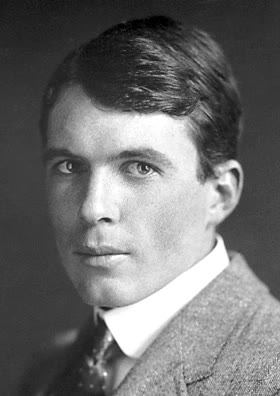
\includegraphics[width=\linewidth]{images/book4/bragg-wl.jpg}\par
{\footnotesize W. L. Bragg.}
\end{minipage}
\end{history}

\section{Ejercicios}

\begin{exercise}[$\star$]\label{exo:b3:x-ray-diffraction:1}
% ledger: lat:NaCl
Para \ce{NaCl} ($a = \qty{564.06}{pm}$), calcúlense $d_{111}$, $d_{200}$ y $d_{220}$.
\end{exercise}

\begin{exercise}[$\star$]\label{exo:b3:x-ray-diffraction:2}
% ledger: lat:Cu, xray:CuKa1
El cobre es FCC con $a = \qty{361.50}{pm}$. Con Cu K$\alpha_1$ ($\lambda = \qty{154.06}{pm}$),
calcúlese el $2\theta$ de sus dos primeras reflexiones, tras nombrarlas.
\end{exercise}

\begin{exercise}[$\star$]\label{exo:b3:x-ray-diffraction:3}
¿Cuáles de las reflexiones 100, 110, 111, 200, 210, 211, 220 están presentes para una
red cúbica P, I y F?
\end{exercise}

\begin{exercise}[$\star$]\label{exo:b3:x-ray-diffraction:4}
Dese la base recíproca de una red rectangular bidimensional de lados
$a$ y $b$, y dibújense los primeros nodos recíprocos.
\end{exercise}

\begin{exercise}[$\star\star$]\label{exo:b3:x-ray-diffraction:5}
% ledger: lat:W
Un metal da rayas a $2\theta = 40.27$, 58.26, 73.20, 87.01 y \ang{100.66} con Cu
K$\alpha_1$. Indéxese el diagrama y encuéntrense el tipo de red y $a$.
\end{exercise}

\begin{exercise}[$\star\star$]\label{exo:b3:x-ray-diffraction:6}
% ledger: lat:KCl
Un cristal de \ce{KCl} ($a = \qty{629.29}{pm}$) tiene una densidad medida de
\qty{1.99}{g/cm^3} (datos del ejercicio). Encuéntrese $Z$.
\end{exercise}

\begin{exercise}[$\star\star$]\label{exo:b3:x-ray-diffraction:7}
La raya (200) de un nanopolvo de \ce{NaCl} ($2\theta = \ang{31.70}$) tiene una anchura de \ang{0.40},
sin contribución del instrumento. Estímese el tamaño de los cristalitos.
\end{exercise}

\begin{exercise}[$\star\star$]\label{exo:b3:x-ray-diffraction:8}
\ce{CsCl} tiene \ce{Cs+} en $(0,0,0)$ y \ce{Cl-} en $(\frac12,\frac12,\frac12)$ en una celda P. Con $f
\approx$ el número de electrones, calcúlense $F_{100}$ y $F_{110}$ y la razón de sus
intensidades (solo el \omterm{def:b3:x-ray-diffraction:structure-factor}{factor de estructura}). ¿Por qué \ce{CsCl} no es centrado en el cuerpo?
\end{exercise}

\begin{exercise}[$\star\star$]\label{exo:b3:x-ray-diffraction:9}
Demuéstrese que una red centrada C (nodo adicional en $(\frac12,\frac12,0)$) hace que falten las
reflexiones con $h + k$ impar.
\end{exercise}

\begin{exercise}[$\star\star\star$]\label{exo:b3:x-ray-diffraction:10}
Explíquese por qué el descubrimiento, en la década de 1980, de aleaciones cuyos diagramas de difracción muestran
manchas nítidas con simetría de orden diez no contradijo la restricción
cristalográfica, y qué cambió en la definición de cristal.
\end{exercise}

\begin{exercise}[$\star\star\star$]\label{exo:b3:x-ray-diffraction:11}
Demuéstrese que en \textit{P}$2_1/c$ el \omterm{def:b3:x-ray-diffraction:space-group}{plano de deslizamiento} hace que falten las reflexiones $h0l$ con $l$
impar.
\end{exercise}

\begin{exercise}[$\star\star\star$]\label{exo:b3:x-ray-diffraction:12}
Un enantiómero puro nunca puede cristalizar en un \omterm{def:b3:x-ray-diffraction:space-group}{grupo espacial} que contenga un
\omterm{def:b3:point-groups:inversion}{centro de inversión}, un \omterm{def:b3:point-groups:mirror}{plano de simetría} o un \omterm{def:b3:x-ray-diffraction:space-group}{plano de deslizamiento}. ¿Por qué? ¿A qué tipo de \omterm{def:b3:x-ray-diffraction:space-group}{grupos espaciales}
está restringido, y qué implica la ley de Friedel para la determinación de su configuración
absoluta?
\end{exercise}

% keep the heading with its problem box, which fills a page by itself
\clearpage
\enlargethispage{3\baselineskip}
\section{Problema: ¿qué polvo blanco?}

\begin{problem}[{Problema de fin de semana --- el diagrama de polvo de una sal cúbica desconocida:
distancias, indexación, el parámetro de red y la identidad de la sal, y el
tamaño de sus cristalitos}]
\label{pb:b3:x-ray-diffraction:1}
% ledger: xray:CuKa1, lat:NaCl, lat:KCl, lat:KBr
Un polvo cristalino blanco desconocido, del que se sabe que es \ce{NaCl}, \ce{KCl} o \ce{KBr},
da con la radiación Cu K$\alpha_1$ ($\lambda = \qty{154.059}{pm}$) las rayas (datos del
problema, calculados para este ejercicio):
\begin{center}\small
\begin{tabular}{lcccccc}
\hline
$2\theta$ / grado & 28.342 & 40.512 & 50.178 & 58.632 & 66.380 & 73.692 \\
intensidad relativa & 100 & 92 & 38 & 20 & 61 & 49 \\ \hline
\end{tabular}
\end{center}
No aparece ninguna otra raya entre 20 y \ang{75}. Parámetros de red de referencia:
\ce{NaCl} \qty{564.06}{pm}, \ce{KCl} \qty{629.29}{pm}, \ce{KBr} \qty{658.47}{pm}. Masas molares:
K 39.1, Na 23.0, Cl 35.5, Br \qty{79.9}{g/mol}.

\medskip\noindent\textbf{Parte I --- Distancias.}
\begin{enumerate}
  \item Calcúlense $\theta$ y $d$ para la primera raya.
  \item Calcúlese $d$ para todas las rayas.
  \item Calcúlense las razones $\sin^2\theta/\sin^2\theta_1$.
  \item ¿Qué serie de enteros se obtiene?
  \item ¿Podría ser el diagrama de una red cúbica primitiva? ¿Con qué $a$?
  \item Para una red cúbica primitiva, ¿qué entero $N$ no puede aparecer nunca? ¿Permite
        el diagrama, hasta aquí, distinguir entre las dos interpretaciones?
\end{enumerate}

\medskip\noindent\textbf{Parte II --- La red real.}
\begin{enumerate}[resume]
  \item Los tres candidatos son redes F. Indéxense las rayas con la serie F.
  \item Dedúzcase $a$ a partir de la primera raya.
  \item ¿Qué candidato se ajusta?
  \item Para esa sal, ¿por qué faltan las reflexiones de índices todos impares (111), (311)?
  \item ¿Mostraría (111) el \ce{NaCl}? ¿Y el \ce{KBr}?
  \item Explíquese por qué la interpretación primitiva de la Parte I es una trampa.
\end{enumerate}

\medskip\noindent\textbf{Parte III --- Densidad y contenido.}
\begin{enumerate}[resume]
  \item ¿Cuántas unidades fórmula contiene la celda?
  \item Calcúlese la densidad a partir de la celda.
  \item Dese el número de coordinación de cada ion.
  \item Calcúlese la distancia K--Cl más corta.
  \item ¿Qué reflexión aparecería primero por encima de \ang{75}?
  \item ¿Por qué las intensidades son menos útiles que las posiciones para identificar una fase?
\end{enumerate}

\medskip\noindent\textbf{Parte IV --- Afinamiento y tamaño de los cristalitos.}
\begin{enumerate}[resume]
  \item ¿Por qué se calcula mejor el parámetro de red a partir de una raya de ángulo alto?
  \item Calcúlese $a$ a partir de la raya (420).
  \item La raya (420) tiene una anchura de \ang{0.25} en $2\theta$ (anchura instrumental
        despreciable). Estímese el tamaño de los cristalitos.
  \item ¿Ensancharía la raya de forma medible un tamaño de cristalito de \qty{1}{\micro m}?
  \item Enúnciese el resultado: el parámetro de red afinado a partir de la raya (420), y
        la identidad del polvo.
\end{enumerate}
\end{problem}
